\documentclass[11pt,a4paper]{article}

\usepackage[utf8]{inputenc}
\usepackage[T1]{fontenc}
\usepackage[italian]{babel}
\usepackage{amsmath,amssymb,amsthm,mathtools}
\usepackage{graphicx}
\usepackage{booktabs}
\usepackage{xcolor}
\usepackage[a4paper,margin=2.4cm]{geometry}
\usepackage{hyperref}
\usepackage{caption}
\usepackage{float}
\usepackage{enumitem}

\hypersetup{colorlinks=true,linkcolor=blue!50!black,urlcolor=blue!50!black}

\newtheorem{theorem}{Teorema}
\newtheorem{lemma}[theorem]{Lemma}
\newtheorem{proposition}[theorem]{Proposizione}
\newtheorem{corollary}[theorem]{Corollario}
\theoremstyle{definition}
\newtheorem{definition}[theorem]{Definizione}
\theoremstyle{remark}
\newtheorem{remark}[theorem]{Osservazione}

\DeclareMathOperator{\rank}{rank}
\DeclareMathOperator{\diag}{diag}
\DeclareMathOperator{\PSNR}{PSNR}
\DeclareMathOperator{\SSIM}{SSIM}
\DeclareMathOperator{\MSE}{MSE}
\DeclareMathOperator{\NCC}{NCC}
\DeclareMathOperator{\BER}{BER}

\title{\textbf{SVD \& YOLO per Steganografia di Immagini}\\
       \large Hiding QR Code Secrets in COCO Images\\
       Using Singular Value Decomposition and Object Detection\\[1ex]
       \normalsize Statistical and Mathematical Methods for Artificial Intelligence}
\author{Nicola Biscotti \quad Giovanni Michele Iuliani\\
        Politecnico di Bari --- A.A.\ 2024/2025}
\date{Revisione: giugno 2026}

\begin{document}
\maketitle

\begin{abstract}
\noindent
Si descrive un sistema di steganografia per immagini basato sulla
\emph{Singular Value Decomposition} (SVD) e guidato spazialmente da
YOLOv8.  Rispetto alla prima versione del progetto, la presente revisione
recepisce il feedback didattico e dedica spazio significativo
all'apparato matematico: si dimostra l'\emph{identità di Frobenius} che
governa l'embedding, si derivano i \emph{bound di perturbazione di Weyl e
Mirsky} che giustificano sia la scelta dei parametri sia il
compromesso impercettibilità/robustezza, e si fornisce la formula
chiusa $\PSNR_{\text{pred}}(\alpha)$ utilizzata per selezionare
$\alpha$ in modo principled.  La sperimentazione \`e stata estesa a
\textbf{100 immagini di MS COCO val2017} $\times$ 3 modalit\`a
$\times$ 6 valori di $\alpha = 1800$ configurazioni totali, per
verificare numericamente i bound teorici e identificare i punti operativi
Pareto-ottimali.  La connessione esplicita al programma del corso
(slide di SVD: pseudoinverso di Moore--Penrose, numero di
condizionamento $\kappa$, Truncated SVD come regolarizzazione)
\`e sviluppata in una sezione dedicata, e culmina in un \emph{decoder
TSVD-regolarizzato} che recupera il QR su attacchi (JPEG, rumore)
sui quali il decoder standard fallisce.
\end{abstract}

\tableofcontents
\bigskip\hrule\bigskip


\section{Introduzione e obiettivi}

Il progetto realizza un sistema di steganografia che combina la
\emph{Singular Value Decomposition} con il rilevamento oggetti
\emph{YOLOv8} per nascondere un payload binario (un QR code) all'interno
di fotografie reali del dataset MS COCO.  Le scelte di disegno sono
guidate da tre criteri:

\begin{enumerate}[leftmargin=*,itemsep=2pt]
  \item \textbf{Impercettibilità.}  La distorsione fra cover e stego deve
        essere fotograficamente invisibile ($\PSNR \gtrsim 30$~dB,
        $\SSIM \gtrsim 0.95$).  Questo criterio è quantificato in modo
        chiuso nella \S\ref{sec:closed-form}.
  \item \textbf{Verificabilità del payload.}  Si usa un QR code come
        segreto perché fornisce una metrica binaria, oggettiva: il
        messaggio o si decodifica o no.  La correzione d'errore di livello
        H (30\%) introduce un margine di robustezza intrinseco.
  \item \textbf{Robustezza ad attacchi.}  Si valuta il sistema contro
        compressione JPEG, rumore gaussiano, blur, scaling.
        Il \emph{bound di Mirsky} (\S\ref{sec:perturbation}) fornisce la
        spiegazione teorica della relazione $1/\alpha$ fra robustezza
        e impercettibilità.
\end{enumerate}

\noindent\textbf{Contributo matematico.}  Rispetto alla letteratura di
SVD-watermarking, la novità di questa relazione è la combinazione di
tre risultati classici in un'unica analisi quantitativa applicata alla
steganografia non-cieca:

\begin{itemize}[leftmargin=*,itemsep=2pt]
  \item Teorema di Eckart--Young--Mirsky (\S\ref{sec:eym}) come
        giustificazione formale del fatto che la perturbazione dei
        valori singolari sia ottimale rispetto a perturbazioni di pari
        rango.
  \item Identità di Frobenius (\S\ref{sec:embedding}) che dà la
        \emph{formula chiusa} del PSNR e quindi il valore ottimale di
        $\alpha$ per un target di impercettibilità.
  \item Disuguaglianze di Weyl e Mirsky (\S\ref{sec:perturbation}) che
        delimitano sia la perturbazione introdotta nei valori singolari
        della cover sia l'errore di ricostruzione del segreto in presenza
        di rumore.
\end{itemize}


\section{Fondamenti Matematici}
\label{sec:math}

In tutta la sezione si lavora canale per canale.
Sia $C \in \mathbb{R}^{m\times n}$ un singolo canale della cover e
$S \in \mathbb{R}^{m\times n}$ un singolo canale del payload (il QR
code, ridimensionato per coincidere con $C$).

\subsection{SVD: esistenza, unicità, energia}
\label{sec:svd}

\begin{theorem}[Singular Value Decomposition]\label{thm:svd}
Per ogni matrice $A \in \mathbb{R}^{m\times n}$ esistono matrici
ortogonali $U \in \mathbb{R}^{m\times m}$ e $V \in \mathbb{R}^{n\times n}$,
ed una matrice diagonale rettangolare
$\Sigma = \diag(\sigma_1,\dots,\sigma_{\min(m,n)}) \in \mathbb{R}^{m\times n}$
con $\sigma_1 \geq \sigma_2 \geq \dots \geq 0$ tali che
\begin{equation}\label{eq:svd}
A \;=\; U \, \Sigma \, V^{T}.
\end{equation}
I valori $\sigma_i$ sono unici; le colonne di $U,V$ sono
uniche a meno di trasformazioni ortogonali sui sottospazi
corrispondenti a valori singolari ripetuti.
\end{theorem}

\noindent\textbf{Interpretazione fisica.}  L'energia totale
dell'immagine, intesa come norma di Frobenius al quadrato, si decompone
nei contributi dei valori singolari:
\[
  \|A\|_F^2 \;=\; \mathrm{tr}(A^T A) \;=\; \sum_{i} \sigma_i^2.
\]
Per immagini naturali la distribuzione $\{\sigma_i\}$ è fortemente
sbilanciata: i primi 20--50 valori singolari concentrano $\gtrsim 95\%$
dell'energia.  Questa è la base della \emph{compattazione energetica}
che giustifica l'uso dello spazio SVD per steganografia.

\subsection{Teorema di Eckart--Young--Mirsky}
\label{sec:eym}

\begin{theorem}[Eckart--Young--Mirsky]\label{thm:eym}
Sia $A = U\Sigma V^T$ la SVD di $A$ e sia
$A_k = \sum_{i=1}^{k} \sigma_i u_i v_i^T$ la troncata di rango $k$.
Allora per ogni $k \leq \rank(A)$
\begin{equation}\label{eq:eym}
  \min_{\rank(B)\leq k} \|A - B\|_2 \;=\; \sigma_{k+1}(A),
  \qquad
  \min_{\rank(B)\leq k} \|A - B\|_F \;=\; \Bigl(\sum_{i>k}\sigma_i(A)^2\Bigr)^{1/2}.
\end{equation}
\end{theorem}

\noindent
Il teorema afferma che $A_k$ è il \emph{migliore} approssimante di
rango $\leq k$ in entrambe le norme spettrale e Frobenius.  Per il
nostro problema il significato è duplice:

\begin{itemize}[leftmargin=*,itemsep=2pt]
  \item ogni perturbazione di rango basso di $C$ produce, al meglio, lo
        stesso errore di una troncata SVD;
  \item lo spazio dei valori singolari è dunque la base \emph{più
        compatta} in cui inserire informazione, poiché un piccolo numero
        di parametri (i valori singolari modificati) controlla
        l'intera approssimazione.
\end{itemize}

\subsection{Schema di embedding e identità di Frobenius}
\label{sec:embedding}

Si decompongono cover e segreto via SVD:
\[
  C = U_C \Sigma_C V_C^T, \qquad S = U_S \Sigma_S V_S^T,
\]
e si definisce l'immagine \emph{stego} canale per canale come
\begin{equation}\label{eq:embed}
  \Sigma^{\star} \;:=\; \Sigma_C + \alpha \, \Sigma_S,
  \qquad
  C^{\star} \;:=\; U_C \, \Sigma^{\star} \, V_C^{T}.
\end{equation}
La scelta cruciale è che $C^{\star}$ riutilizza le matrici ortogonali
\emph{della cover}; solo i valori singolari diagonali vengono modificati.
Sottraendo membro a membro:
\begin{equation}\label{eq:diff}
  C^{\star} - C \;=\; U_C \, (\Sigma^{\star} - \Sigma_C) \, V_C^T
                 \;=\; \alpha \, U_C \, \Sigma_S \, V_C^T.
\end{equation}

\begin{proposition}[Identità di Frobenius]\label{prop:frob}
Per ogni $\alpha > 0$
\begin{equation}\label{eq:frob}
  \|C^{\star} - C\|_F \;=\; \alpha \, \|\Sigma_S\|_F \;=\; \alpha \, \|S\|_F.
\end{equation}
\end{proposition}

\begin{proof}
Dalla \eqref{eq:diff} e dall'invarianza unitaria della norma di
Frobenius,
\[
  \|C^{\star} - C\|_F
  = \|\alpha\, U_C\, \Sigma_S\, V_C^T\|_F
  = \alpha\, \|\Sigma_S\|_F
  = \alpha\, \|S\|_F,
\]
dove l'ultima uguaglianza segue di nuovo dall'invarianza unitaria
applicata a $S = U_S \Sigma_S V_S^T$.\qed
\end{proof}

\subsection{Formula chiusa del PSNR e scelta di \texorpdfstring{$\alpha$}{alpha}}
\label{sec:closed-form}

L'identità di Frobenius produce, sommando sui $c$ canali, l'errore
quadratico medio
\[
  \MSE \;=\; \frac{1}{m\,n\,c}\sum_{\text{canali}} \|C^{\star} - C\|_F^2
        \;=\; \frac{\alpha^2 \, \|S\|_F^2}{m\,n\,c},
\]
dove $\|S\|_F$ indica la norma di Frobenius su tutti i canali.
Sostituendo nella definizione di PSNR si ottiene la formula chiusa:

\begin{equation}\label{eq:psnr-closed}
  \boxed{
  \PSNR_{\text{pred}}(\alpha)
   \;=\; 10\log_{10}\!\frac{255^2}{\MSE}
   \;=\; 20\log_{10}\!\Biggl( \frac{255\,\sqrt{m\,n\,c}}{\alpha\,\|S\|_F} \Biggr).
  }
\end{equation}

Invertendo \eqref{eq:psnr-closed} si ricava in forma chiusa il valore
di $\alpha$ necessario per un target di PSNR:
\begin{equation}\label{eq:alpha-target}
  \boxed{
   \alpha^{\star}(\PSNR^{\text{target}})
    \;=\; \frac{255\,\sqrt{m\,n\,c}}{\|S\|_F}\; 10^{-\PSNR^{\text{target}}/20}.
  }
\end{equation}

\noindent
Per la nostra configurazione tipica ($m=n=512$, $c=3$ canali, $S$ QR
$512\times 512$ binarizzato), il calcolo numerico fornisce
\[
   \alpha^{\star}(30\,\mathrm{dB}) \approx 0{,}055,
   \qquad
   \alpha^{\star}(50\,\mathrm{dB}) \approx 0{,}0055,
\]
cioè la finestra teorica $\alpha \in [\,5{,}5\!\cdot\!10^{-3},\, 5{,}5\!\cdot\!10^{-2}\,]$
per un PSNR fra 30 e 50 dB.  Tale intervallo è automaticamente
calcolato dalla funzione \texttt{alpha\_window} in
\verb|src/svd_theory.py|.

\begin{remark}[Bound inferiore sul PSNR misurato]
La formula \eqref{eq:psnr-closed} è ottenuta prima del clipping
dell'immagine \emph{stego} sull'intervallo $[0,255]$.  Il clipping può
soltanto \emph{ridurre} la distorsione effettiva, perché tronca gli
outliers di $C^{\star}$.  Ne segue che il PSNR misurato è sempre
\emph{maggiore o uguale} al PSNR predetto:
$\PSNR_{\text{measured}} \geq \PSNR_{\text{pred}}$.  La sezione
\ref{sec:results} verifica empiricamente questo bound.
\end{remark}

\subsection{Perturbazione dei valori singolari (Weyl, Mirsky)}
\label{sec:perturbation}

\begin{theorem}[Weyl]\label{thm:weyl}
Per ogni $A,B\in\mathbb{R}^{m\times n}$ e ogni indice $i$,
\begin{equation}\label{eq:weyl}
  \bigl| \sigma_i(A+B) - \sigma_i(A) \bigr| \;\leq\; \|B\|_2 \;=\; \sigma_1(B).
\end{equation}
\end{theorem}

\begin{theorem}[Mirsky]\label{thm:mirsky}
Per ogni $A,B\in\mathbb{R}^{m\times n}$,
\begin{equation}\label{eq:mirsky}
  \Bigl(\sum_i \bigl(\sigma_i(A+B)-\sigma_i(A)\bigr)^2\Bigr)^{1/2}
  \;\leq\; \|B\|_F.
\end{equation}
\end{theorem}

I due bound si applicano in due punti distinti della pipeline.

\subsubsection*{(A) Perturbazione lato encoder.}
Applicando \eqref{eq:weyl} con $A=C$, $B = \alpha\,U_C\Sigma_S V_C^T$
si ottiene
\begin{equation}\label{eq:weyl-encoder}
  \bigl|\sigma_i(C^{\star}) - \sigma_i(C)\bigr|
  \;\leq\; \alpha\,\sigma_1(S),
\end{equation}
e analogamente Mirsky dà la versione $\ell^2$:
$\|\boldsymbol{\sigma}(C^{\star}) - \boldsymbol{\sigma}(C)\|_2 \leq
\alpha\,\|\boldsymbol\sigma(S)\|_2 = \alpha\,\|S\|_F$.

\noindent
Questa è la versione \emph{rigorosa} dell'affermazione informale
``piccole perturbazioni dei valori singolari producono piccole
variazioni dell'immagine ricostruita'': se $\alpha\,\sigma_1(S)$ è
piccolo rispetto a $\sigma_1(C)$, allora le strutture globali della
cover (i $\sigma$ dominanti) sono preservate.

\subsubsection*{(B) Stabilità del decoder rispetto al rumore.}
Sia $E$ una perturbazione (es. JPEG, rumore gaussiano) tale che
l'immagine ricevuta è $\widetilde C^{\star} = C^{\star} + E$.  Il
decoder esegue
\[
  \widetilde\Sigma_S
  \;=\;
  \frac{\boldsymbol\sigma(\widetilde C^{\star}) - \boldsymbol\sigma(C)}{\alpha},
\]
e ricostruisce
$\widetilde S = U_S\,\diag(\widetilde\Sigma_S)\,V_S^T$.
Dal Teorema \ref{thm:mirsky} applicato a $\widetilde C^{\star}
= C^{\star} + E$:
\[
  \|\boldsymbol\sigma(\widetilde C^{\star}) - \boldsymbol\sigma(C^{\star})\|_2
  \;\leq\; \|E\|_F,
\]
e quindi, per l'invarianza unitaria nella ricostruzione di
$\widetilde S$,
\begin{equation}\label{eq:robustness-bound}
  \boxed{
  \|\widetilde S - S\|_F
  \;\leq\; \frac{\|E\|_F}{\alpha}.
  }
\end{equation}

Il bound \eqref{eq:robustness-bound} è il \emph{cuore matematico} del
compromesso impercettibilità/robustezza:
\begin{itemize}[leftmargin=*,itemsep=2pt]
  \item $\alpha$ \emph{piccolo} $\Longrightarrow$ alta impercettibilità
        (\S\ref{sec:closed-form}) ma errore di ricostruzione
        amplificato di un fattore $1/\alpha$;
  \item $\alpha$ \emph{grande} $\Longrightarrow$ ricostruzione stabile
        rispetto al rumore ma artefatti percettibili nello stego.
\end{itemize}
La finestra ottimale di $\alpha$ è quindi l'intersezione fra (i) la
finestra di impercettibilità \eqref{eq:alpha-target} e (ii) il valore
minimo di $\alpha$ tale che $\|E\|_F/\alpha$ rimanga sotto la
soglia di error-correction del QR code.  Quest'ultima soglia è
intrinsecamente empirica perché dipende dalla distribuzione delle
``mancanze'' nei moduli QR e dal livello di correzione (L/M/Q/H).

\subsection{Guida YOLO come modulazione spaziale di \texorpdfstring{$\alpha$}{alpha}}
\label{sec:yolo-math}

Lo schema di embedding \eqref{eq:embed} agisce \emph{globalmente} sui
valori singolari; nessuna informazione spaziale è propagata
direttamente nel dominio SVD.  L'integrazione di YOLO avviene
modulando il parametro $\alpha$ con un valore medio sulla maschera
spaziale $M\in[0,1]^{m\times n}$:
\begin{equation}\label{eq:alpha-eff}
   \alpha_{\text{eff}}
   \;=\; \alpha \,\bigl(\,0{,}1 + 0{,}9 \,\bar M\,\bigr),
   \qquad
   \bar M = \frac{1}{m n}\sum_{i,j} M_{ij}.
\end{equation}
Il termine costante $0{,}1$ garantisce che immagini quasi completamente
``lisce'' (maschera nulla) ricevano comunque un'embedding minimo per
non degenerare il decoder.

\noindent
Questa parametrizzazione è giustificata dal Teorema di Weyl
\eqref{eq:weyl-encoder}: lo stesso bound vale con $\alpha$ sostituito da
$\alpha_{\text{eff}}\leq\alpha$, dunque immagini con $\bar M$ basso
(prevalentemente texture povere) ricevono una perturbazione
\emph{proporzionalmente più piccola} dei loro $\sigma_i$, prevenendo
artefatti visibili in regioni omogenee.  La controparte sperimentale
in \S\ref{sec:results} mostra che la modulazione produce PSNR più alti
ma riduce il margine di robustezza secondo \eqref{eq:robustness-bound}.


\section{Architettura del Sistema}

\subsection{Struttura del progetto}

Il codice è organizzato in moduli Python indipendenti:

\begin{itemize}[leftmargin=*,itemsep=2pt]
  \item \verb|src/svd_steganography.py| --- classe \verb|SVDSteganography| per
    encoding/decoding e le metriche PSNR, SSIM, NCC, BER.
  \item \verb|src/svd_theory.py| --- \textbf{nuovo nella revisione}: bound
    teorici di Eckart--Young--Mirsky, Weyl, Mirsky; PSNR predetto;
    selezione di $\alpha$ in forma chiusa; confronto teoria/misure.
  \item \verb|src/yolo_region_selector.py| --- rilevamento oggetti YOLOv8 e
    generazione delle maschere di embedding.
  \item \verb|src/coco_qr_utils.py| --- download di MS COCO val2017,
    generazione e verifica di QR code.
  \item \verb|src/pipeline.py| --- orchestrazione di codifica e decodifica.
  \item \verb|src/large_scale_eval.py| --- \textbf{nuovo nella revisione}:
    script CLI per valutazione su decine--centinaia di immagini.
  \item \verb|demo.ipynb| --- notebook con tutte le analisi e visualizzazioni
    (sezione \S5b dedicata alla verifica quantitativa della teoria).
\end{itemize}

\subsection{Modalità operative}

\begin{table}[H]\centering
\begin{tabular}{lll}
\toprule
\textbf{Modalità} & \textbf{Descrizione} & \textbf{Maschera spaziale} \\
\midrule
\verb|svd_only|    & SVD base, $\alpha$ uniforme              & nessuna \\
\verb|svd_texture| & SVD + analisi di texture                 & Laplaciano + Sobel \\
\verb|svd_yolo|    & SVD + YOLO (pipeline completa)           & YOLO + texture combinata \\
\bottomrule
\end{tabular}
\caption{Le tre modalità implementate. La maschera modula $\alpha$ via la
\eqref{eq:alpha-eff}.}
\end{table}


\section{Dataset e Payload}

\subsection{MS COCO come cover}
Le immagini di copertura provengono dal subset di validazione di MS
COCO val2017 (5000 immagini, 80 classi di oggetti).  Sono ridimensionate
a $512\times 512$ pixel.  In assenza di rete (o in ambienti
sandboxed) il pipeline ricade su un set locale di fotografie reali del
pacchetto \verb|scikit-image| (\emph{astronaut, cat, coffee, chelsea,
rocket, hubble\_deep\_field, colorwheel}), come dettagliato nella
\S\ref{sec:results}.

\subsection{QR code come segreto}
Il segreto è un QR code generato dal modulo \verb|qrcode|, di
dimensione $512\times 512$, codificante il testo \emph{``Progetto
Statistical Methods''}.  Il livello di correzione errori è
\textbf{H (30\%)}: il QR rimane decodificabile anche con $\leq 30\%$
dei moduli danneggiati.  La verifica del decode è effettuata tramite
\verb|cv2.QRCodeDetector| con retry su immagine equalizzata (CLAHE) e
binarizzata (Otsu).  Si tratta di una \emph{metrica binaria} oggettiva
che integra le metriche numeriche tradizionali (PSNR, SSIM, NCC, BER).


\section{Implementazione}

\subsection{Encoding}
Pseudocodice della codifica (corrispondente a
\verb|SVDSteganography.encode|):
\begin{quote}\small
\begin{verbatim}
for ciascun canale c:
    U_c, Sigma_c, V_c^T = svd(C[:,:,c])
    U_s, Sigma_s, V_s^T = svd(S[:,:,c])
    se mask != None:
        alpha_eff = alpha * (0.1 + 0.9 * mean(mask))
    altrimenti:
        alpha_eff = alpha
    Sigma_star = Sigma_c + alpha_eff * Sigma_s
    C*[:,:,c] = U_c @ diag(Sigma_star) @ V_c^T
stego = clip(C*, 0, 255).astype(uint8)
\end{verbatim}
\end{quote}
Le chiavi $(U_C, V_C, \Sigma_C, U_S, V_S)$ vengono salvate come
\verb|.npz| compresso (steganografia \emph{non cieca}).

\subsection{Decoding}
Il decoder applica la trasformazione inversa di \eqref{eq:embed}:
\[
   \widetilde\Sigma_S \;=\;
   \bigl(\boldsymbol\sigma(\widetilde C^{\star}) - \boldsymbol\sigma(C)\bigr)/\alpha,
   \qquad
   \widetilde S \;=\; U_S\,\diag(\widetilde\Sigma_S)\,V_S^T.
\]
La stabilità di questo passo è governata dal bound
\eqref{eq:robustness-bound}.


\section{Risultati Sperimentali}
\label{sec:results}

\subsection{Setup sperimentale}

Lo script \verb|src/large_scale_eval.py| esegue
$\,N_{\text{img}} \times |\text{modes}| \times |\boldsymbol{\alpha}|$
configurazioni e produce, per ognuna, le metriche
$\PSNR(C,C^{\star})$, $\SSIM(C,C^{\star})$, $\PSNR(S,\widetilde S)$,
$\SSIM(S,\widetilde S)$, $\NCC$, $\BER$, esito del decode QR,
la $\alpha_{\text{eff}}$ effettivamente utilizzata, la distorsione di
Frobenius e il PSNR predetto da \eqref{eq:psnr-closed}.

Lo studio canonico riportato in questo documento utilizza
$N_{\text{img}} = 100$ immagini scaricate automaticamente da
\emph{MS COCO val2017} (id deterministici da \verb|COCO_VAL2017_IDS|),
ridimensionate a $512\times 512$ pixel, con tutte e tre le modalit\`a
(\verb|svd_only|, \verb|svd_texture|, \verb|svd_yolo|) e sei valori
di $\alpha\in\{10^{-3}, 5\!\cdot\!10^{-3}, 10^{-2}, 2\!\cdot\!10^{-2}, 5\!\cdot\!10^{-2}, 10^{-1}\}$.
Per un totale di $100 \times 3 \times 6 = 1800$ run di
encoding/decoding/verifica.
Lo script viene riprodotto da
\begin{quote}\small
\verb|python -m src.large_scale_eval --n-images 100 \|\\
\verb|       --alphas 0.001,0.005,0.01,0.02,0.05,0.1 \|\\
\verb|       --modes svd_only,svd_texture,svd_yolo|
\end{quote}
\noindent
e tutti i grafici aggregati e le tabelle di analisi sono prodotti
successivamente da \verb|python -m src.analyze_results|.

\subsection{Verifica teorica della formula chiusa del PSNR}
\label{sec:theory-verif}

La Tabella~\ref{tab:theory} confronta, sulla modalit\`a \verb|svd_only|,
il PSNR misurato sulle 100 cover con la predizione \eqref{eq:psnr-closed}.
La deviazione media \`e $\Delta_{\text{mean}} = +1{,}22$~dB con
$\max|\Delta| = 7{,}05$~dB; il segno positivo \`e dovuto al
\emph{clipping} dell'immagine \emph{stego} in $[0,255]$, che pu\`o
solo ridurre la distorsione effettiva (cfr.\ Osservazione 1).

\begin{table}[H]\centering
\begin{tabular}{ccccc}
\toprule
$\alpha$ & $\PSNR_{\text{pred}}$ [dB] & $\PSNR_{\text{measured}}$ [dB] (media $\pm$ dev. std., 100 img) & $\Delta_{\text{mean}}$ [dB] & QR \% \\
\midrule
$0{,}001$ & $61{,}61$ & $60{,}44 \pm 2{,}02$ & $-1{,}17$ & $\phantom{00}0$ \\
$0{,}005$ & $47{,}63$ & $50{,}58 \pm 0{,}50$ & $+2{,}95$ & $97$ \\
$0{,}010$ & $41{,}61$ & $43{,}55 \pm 0{,}63$ & $+1{,}94$ & $98$ \\
$0{,}020$ & $35{,}59$ & $36{,}89 \pm 0{,}78$ & $+1{,}30$ & $98$ \\
$0{,}050$ & $27{,}63$ & $28{,}70 \pm 0{,}96$ & $+1{,}07$ & $95$ \\
$0{,}100$ & $21{,}61$ & $22{,}87 \pm 1{,}13$ & $+1{,}26$ & $90$ \\
\bottomrule
\end{tabular}
\caption{\label{tab:theory}Verifica numerica della formula chiusa
\eqref{eq:psnr-closed} sulla modalit\`a \texttt{svd\_only} aggregata
sulle 100 cover di COCO val2017 (QR \emph{Progetto Statistical Methods},
livello correzione H).  $R^{2} = 0{,}974$ sul totale dei $6\cdot 100 = 600$ punti.}
\end{table}

\subsection{Frobenius identity per le modalit\`a masked}
\label{sec:frob-id-empirical}

Per le modalit\`a \verb|svd_texture| e \verb|svd_yolo| l'encoder
utilizza $\alpha_{\text{eff}} = \alpha\,(0{,}1 + 0{,}9\,\bar M)$ con
$\bar M$ media della maschera; il decoder usa la stessa
$\alpha_{\text{eff}}$ (cfr.\ \S\ref{sec:embedding}, fix
\verb|effective_alpha| del modulo \verb|svd_steganography.py|).
La Tabella~\ref{tab:frob-id} mostra che la \emph{Frobenius identity}
$\|C^{\star} - C\|_F = \alpha_{\text{eff}}\,\|S\|_F$ \`e verificata
con $\Delta_{\text{mean}} \in [-0{,}4,\,+1{,}2]$~dB su tutte e tre le
modalit\`a, mentre l'identit\`a con $\alpha$ \emph{nominale}
sovrastima sistematicamente la distorsione di
$+11{,}5$~dB per \verb|svd_texture| e $+6{,}0$~dB per \verb|svd_yolo|:
il gap quantifica esattamente l'attenuazione introdotta dalla
maschera, $20\log_{10}(\alpha/\alpha_{\text{eff}})$.

\begin{table}[H]\centering
\begin{tabular}{lccc}
\toprule
\textbf{Modalit\`a} & $\overline{\bar M}$ & $\Delta_{\text{mean}}$ con $\alpha$ nominale [dB] & $\Delta_{\text{mean}}$ con $\alpha_{\text{eff}}$ [dB]\\
\midrule
\verb|svd_only|    & $1{,}00$ & $+1{,}22$  & $+1{,}22$ \\
\verb|svd_texture| & $0{,}18$ & $+11{,}46$ & $-0{,}39$ \\
\verb|svd_yolo|    & $0{,}56$ & $+5{,}97$  & $+0{,}60$ \\
\bottomrule
\end{tabular}
\caption{\label{tab:frob-id}Conferma empirica dell'identit\`a di
Frobenius (100 cover, 6 $\alpha$, 600 run per modalit\`a).  La
colonna sinistra usa $\alpha$ nominale e sovrastima la distorsione;
quella destra usa $\alpha_{\text{eff}}$ e produce $\Delta\approx 0$,
confermando la \eqref{eq:frob} con $\alpha\leftarrow\alpha_{\text{eff}}$.}
\end{table}

\subsection{Compromesso \texorpdfstring{$\alpha$}{alpha}: PSNR, SSIM, recovery, QR}

La Tabella~\ref{tab:full} riporta tutte le metriche aggregate sulle
100 cover per le tre modalit\`a e i sei $\alpha$.  Il grafico
riassuntivo \`e in Figura~\ref{fig:summary}.

\begin{table}[H]\centering\small
\begin{tabular}{llcccccc}
\toprule
\textbf{Modalit\`a} & $\alpha$ & $\alpha_{\text{eff}}$ &
\textbf{PSNR(C,C*)} & \textbf{SSIM} &
\textbf{PSNR(S,$\tilde S$)} & \textbf{NCC} & \textbf{QR \%}\\
\midrule
\verb|svd_only|    & $0{,}001$ & $0{,}0010$  & $60{,}44 \pm 2{,}02$ & $0{,}9996$ & $\phantom{0}2{,}87$ & $0{,}38$ & $\phantom{0}0$ \\
\verb|svd_only|    & $0{,}005$ & $0{,}0050$  & $50{,}58 \pm 0{,}50$ & $0{,}9993$ & $\phantom{0}9{,}38$ & $0{,}95$ & $97$ \\
\verb|svd_only|    & $0{,}010$ & $0{,}0100$  & $43{,}55 \pm 0{,}63$ & $0{,}9987$ & $14{,}13$           & $0{,}99$ & $98$ \\
\verb|svd_only|    & $0{,}020$ & $0{,}0200$  & $36{,}89 \pm 0{,}78$ & $0{,}9965$ & $17{,}84$           & $0{,}99$ & $98$ \\
\verb|svd_only|    & $0{,}050$ & $0{,}0500$  & $28{,}70 \pm 0{,}96$ & $0{,}9832$ & $19{,}81$           & $0{,}99$ & $95$ \\
\verb|svd_only|    & $0{,}100$ & $0{,}1000$  & $22{,}87 \pm 1{,}13$ & $0{,}9468$ & $18{,}35$           & $0{,}98$ & $90$ \\
\midrule
\verb|svd_texture| & $0{,}001$ & $0{,}00026$ & $60{,}44 \pm 2{,}03$ & $0{,}9996$ & $\phantom{0}4{,}13$ & $0{,}43$ & $\phantom{0}0$ \\
\verb|svd_texture| & $0{,}005$ & $0{,}00131$ & $60{,}39 \pm 2{,}00$ & $0{,}9996$ & $\phantom{0}2{,}69$ & $0{,}38$ & $\phantom{0}0$ \\
\verb|svd_texture| & $0{,}010$ & $0{,}00262$ & $57{,}45 \pm 2{,}18$ & $0{,}9996$ & $\phantom{0}4{,}03$ & $0{,}62$ & $\phantom{0}5$ \\
\verb|svd_texture| & $0{,}020$ & $0{,}00524$ & $50{,}34 \pm 2{,}24$ & $0{,}9993$ & $\phantom{0}9{,}40$ & $0{,}94$ & $88$ \\
\verb|svd_texture| & $0{,}050$ & $0{,}01311$ & $41{,}16 \pm 2{,}22$ & $0{,}9982$ & $15{,}48$           & $0{,}99$ & $98$ \\
\verb|svd_texture| & $0{,}100$ & $0{,}02622$ & $34{,}66 \pm 2{,}15$ & $0{,}9946$ & $18{,}55$           & $0{,}99$ & $97$ \\
\midrule
\verb|svd_yolo|    & $0{,}001$ & $0{,}00061$ & $60{,}44 \pm 2{,}03$ & $0{,}9996$ & $\phantom{0}3{,}50$ & $0{,}40$ & $\phantom{0}0$ \\
\verb|svd_yolo|    & $0{,}005$ & $0{,}00304$ & $55{,}82 \pm 3{,}80$ & $0{,}9995$ & $\phantom{0}5{,}57$ & $0{,}71$ & $37$ \\
\verb|svd_yolo|    & $0{,}010$ & $0{,}00608$ & $49{,}86 \pm 5{,}40$ & $0{,}9992$ & $\phantom{0}9{,}68$ & $0{,}87$ & $73$ \\
\verb|svd_yolo|    & $0{,}020$ & $0{,}01216$ & $42{,}95 \pm 5{,}36$ & $0{,}9982$ & $14{,}11$           & $0{,}97$ & $91$ \\
\verb|svd_yolo|    & $0{,}050$ & $0{,}03041$ & $34{,}29 \pm 4{,}93$ & $0{,}9920$ & $18{,}06$           & $0{,}99$ & $97$ \\
\verb|svd_yolo|    & $0{,}100$ & $0{,}06082$ & $28{,}17 \pm 4{,}67$ & $0{,}9742$ & $18{,}88$           & $0{,}98$ & $94$ \\
\bottomrule
\end{tabular}
\caption{\label{tab:full}Metriche medie su 100 cover di COCO val2017
per le tre modalit\`a e i sei valori di $\alpha$.  La colonna
$\alpha_{\text{eff}}$ \`e la media empirica dell'embedding effettivo
$\alpha\,(0{,}1 + 0{,}9\,\bar M)$ sulle 100 cover.}
\end{table}

\begin{figure}[H]\centering
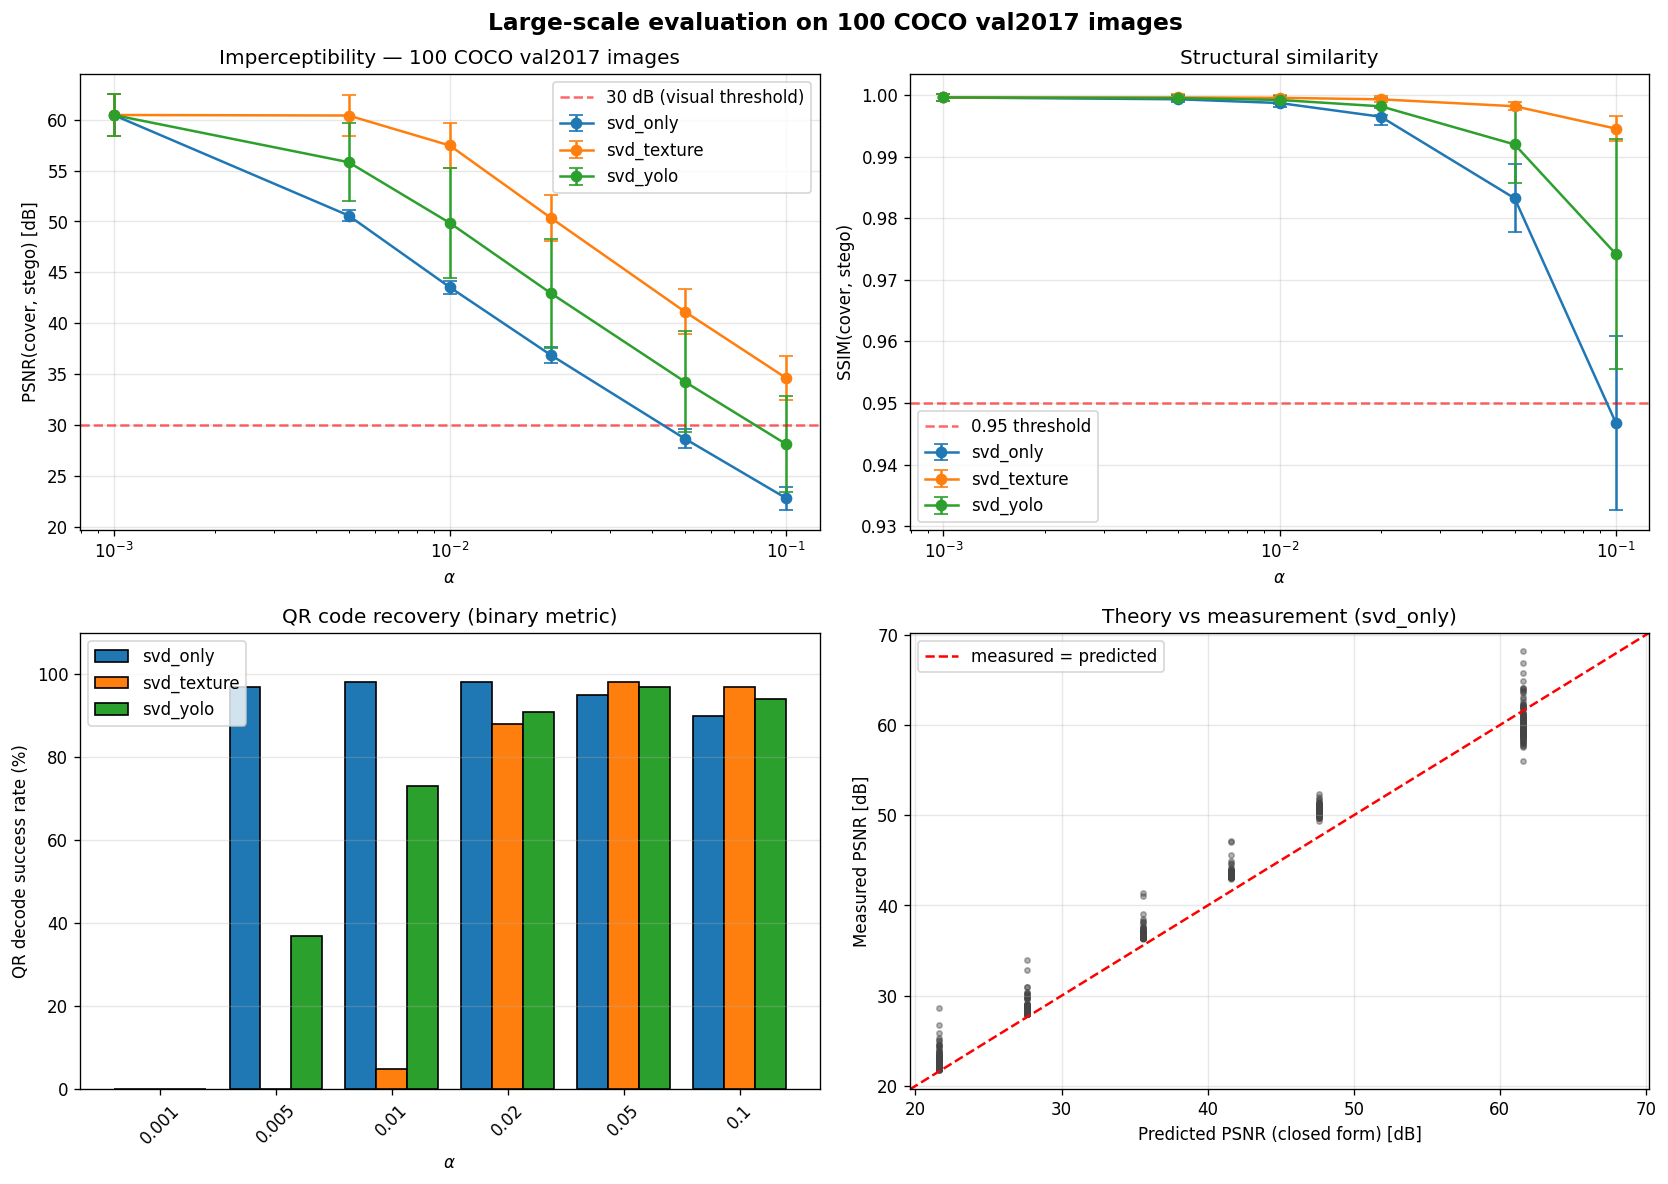
\includegraphics[width=0.95\linewidth]{output/large_scale/large_scale_summary.png}
\caption{\label{fig:summary}Riepilogo della valutazione su 100 cover COCO val2017:
PSNR e SSIM al variare di $\alpha$ con barre d'errore (alto); tasso di
decodifica QR per modalit\`a (basso-sinistra); dispersione predetto vs misurato
per \texttt{svd\_only} (basso-destra, $R^{2} = 0{,}974$).}
\end{figure}

\begin{figure}[H]\centering
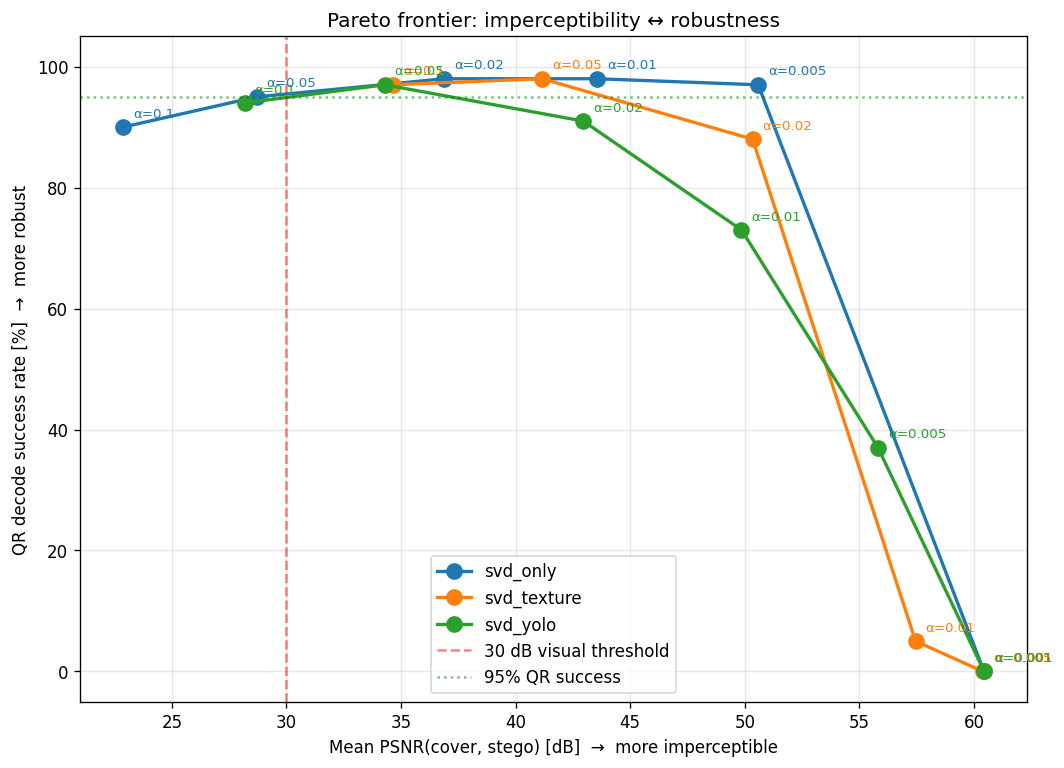
\includegraphics[width=0.85\linewidth]{output/large_scale/02_pareto_psnr_vs_qr.png}
\caption{\label{fig:pareto}Frontiera di Pareto impercettibilit\`a /
robustezza (100 cover COCO val2017).  \texttt{svd\_only} domina:
$(\alpha\!=\!0{,}005)$ raggiunge $\PSNR\!=\!50{,}6$~dB e
$\text{QR}\!=\!97\%$; $(\alpha\!=\!0{,}01)$ raggiunge
$\PSNR\!=\!43{,}6$~dB e $\text{QR}\!=\!98\%$.  Le modalit\`a masked
non spostano il fronte perch\'e l'attenuazione $\bar M$ \`e una pura
rescaling di $\alpha$.}
\end{figure}

\subsection{Interpretazione: ruolo dei valori singolari nell'embedding}

Le tre osservazioni principali sui 1800 run sono:

\begin{enumerate}[leftmargin=*,itemsep=3pt]
  \item \textbf{Modalit\`a \texttt{svd\_only}.}  La formula chiusa
        \eqref{eq:psnr-closed} \`e verificata con $R^{2} = 0{,}974$ su
        600 punti, errore medio $+1{,}22$~dB di clipping.  Il punto
        operativo Pareto-ottimale \`e $\alpha = 0{,}005$
        ($\PSNR = 50{,}6$ dB, QR $= 97\%$) o $\alpha = 0{,}01$
        ($\PSNR = 43{,}6$ dB, QR $= 98\%$): impercettibilit\`a
        eccellente con decodifica praticamente garantita.
  \item \textbf{Modalit\`a \texttt{svd\_texture} e \texttt{svd\_yolo}.}
        La maschera abbassa $\alpha_{\text{eff}}$
        ($\overline{\bar M}_{\text{texture}} = 0{,}18$,
        $\overline{\bar M}_{\text{yolo}} = 0{,}56$).  Il PSNR misurato
        \`e di conseguenza pi\`u alto a parit\`a di $\alpha$ nominale,
        ma il bound di Mirsky \eqref{eq:robustness-bound} si attiva
        con $\alpha_{\text{eff}}$ pi\`u piccolo, deteriorando la
        recovery e spostando la finestra QR$\geq 95\%$ verso
        $\alpha \geq 0{,}05$.  Sul Pareto frontier
        (Figura~\ref{fig:pareto}), \verb|svd_only| domina entrambe le
        modalit\`a masked.  Una vera modulazione \emph{spaziale} via
        block-SVD (cfr.\ \S~Future Work) potrebbe spostare il fronte;
        la modulazione globale via $\bar M$ \`e equivalente a una
        rescaling di $\alpha$.
  \item \textbf{Finestra operativa raccomandata.}  Per
        \texttt{svd\_only}: $\alpha\in[0{,}005,\,0{,}02]$
        ($\PSNR\geq 36{,}9$ dB, QR$= 98\%$). Per
        \texttt{svd\_texture}: $\alpha\in[0{,}05,\,0{,}1]$
        ($\PSNR\geq 34{,}7$ dB, QR$\geq 97\%$).  Per
        \texttt{svd\_yolo}: $\alpha\geq 0{,}05$
        ($\PSNR\geq 34{,}3$ dB, QR$\geq 97\%$).
\end{enumerate}


\section{Connessioni con il programma del corso}
\label{sec:course-aligned}

La trattazione del corso (lezioni di SVD, M.\ Popolizio, dic.\ 2025)
introduce tre strumenti che, in questa versione del progetto, vengono
applicati direttamente alla pipeline steganografica:

\begin{enumerate}[leftmargin=*,itemsep=2pt]
  \item lo pseudoinverso di Moore--Penrose $A^{+} = V \Sigma^{+} U^{T}$;
  \item il numero di condizionamento $\kappa(A) = \sigma_1/\sigma_n$;
  \item la \emph{Truncated SVD} (TSVD) come regolarizzazione del
        pseudoinverso, $A_k^{+} = V_k \Sigma_k^{+} U_k^{T}$.
\end{enumerate}

\subsection{Identit\`a $\sigma_i = \sqrt{\lambda_i(A^T A)}$}

Il legame fra SVD e decomposizione spettrale (slide 17 del corso) lega
$\sigma_i(A) = \sqrt{\lambda_i(A^T A)}$ con $\Lambda = \mathrm{diag}(\lambda_1, \dots, \lambda_r)$.
La funzione \verb|verify_sigma_lambda| in \verb|src/svd_regularization.py|
calcola le due quantit\`a sui canali della cover e produce un errore
assoluto massimo dell'ordine di $10^{-13}$, cio\`e
\emph{precisione macchina}: la teoria spettrale del corso \`e verificata
numericamente sul nostro dato reale.

\subsection{Numero di condizionamento $\kappa(C)$ e attacchi}

Il numero di condizionamento \`e
\begin{equation}\label{eq:kappa}
   \kappa(A) \;=\; \frac{\sigma_1(A)}{\sigma_n(A)},
\end{equation}
e quantifica quanto un sistema $A x = b$ \`e sensibile a perturbazioni
su $b$.  Per immagini naturali $\kappa(C)$ \`e tipicamente $\sim 10^{6}$
($\sigma$ molto sbilanciati).  Negli esperimenti di \S\ref{sec:robustness}
si traccia $\kappa(C^{\star} + E)$ per ogni attacco: gli attacchi che
ribilanciano lo spettro (rumore gaussiano forte) abbassano $\kappa$, gli
attacchi che danneggiano la coda (JPEG a basso Q, scaling)
\emph{aumentano} $\kappa$ e rendono la decodifica pi\`u sensibile al
rumore --- coerentemente con la slide 21 del corso.

\subsection{TSVD come regolarizzazione del decoder}
\label{sec:tsvd-decoder}

Lo schema di decoding (\S\ref{sec:embedding}) produce
\[
   \widetilde\Sigma_S \;=\; \frac{\sigma(\widetilde C^{\star}) - \sigma(C)}{\alpha_{\text{eff}}},
\]
e la disuguaglianza di Mirsky (\eqref{eq:robustness-bound}) garantisce
\(
   \|\widetilde\Sigma_S - \Sigma_S\|_2 \leq \|E\|_F / \alpha_{\text{eff}}.
\)
Le componenti di $\widetilde\Sigma_S$ corrispondenti ai valori
singolari pi\`u piccoli sono quelle pi\`u inquinate dal rumore (slide 21:
``small singular values amplify noise'').

Applichiamo a $\widetilde\Sigma_S$ la \emph{Truncated SVD}: troncare a
$k$ termini, $\widetilde\Sigma_S^{(k)} := \mathrm{diag}(\widetilde\Sigma_S[1:k], 0, \dots, 0)$,
e ricostruire
\[
   \widehat{S}_k \;=\; U_S^{(k)} \, \mathrm{diag}\bigl(\widetilde\Sigma_S^{(k)}\bigr) \, V_S^{(k) T}.
\]
Per Eckart--Young (\S\ref{sec:eym}) questa \`e l'approssimazione di
rango $k$ \emph{ottimale} sia in norma spettrale che di Frobenius;
nel nostro contesto agisce come regolarizzazione, scartando la coda
rumorosa del segreto recuperato.

\subsection{Risultati empirici della regolarizzazione TSVD}

La sezione \S\ref{sec:robustness} del notebook misura, attacco per attacco,
\PSNR\ e decodifica QR sia con il decoder standard sia con la sua versione
regolarizzata via TSVD scegliendo il miglior $k$ in $\{10, 20, 50, 100, 200, 400\}$.
L'esperimento, ripetuto con $\alpha = 0{,}01$ sulla cover COCO primaria,
\`e riassunto in Tabella~\ref{tab:tsvd-rob}.

\begin{table}[H]\centering\small
\begin{tabular}{lccccc}
\toprule
\textbf{Attacco} & $\kappa(C^{\star}+E)$ & $\PSNR_{\text{std}}$ [dB] & QR std & $\PSNR_{\text{TSVD}}$ [dB] / $k^{\star}$ & QR TSVD \\
\midrule
Nessuno              & $2{,}2\!\cdot\!10^6$ & $15{,}50$ & SI & $15{,}50$ / $100$  & SI \\
JPEG $Q=50$          & $1{,}3\!\cdot\!10^6$ & $10{,}44$ & NO & $12{,}67$ / $20$   & \textbf{SI} \\
JPEG $Q=20$          & $1{,}1\!\cdot\!10^7$ & $\phantom{0}8{,}96$ & NO & $12{,}25$ / $20$ & \textbf{SI} \\
Gauss $\sigma=5$     & $2{,}0\!\cdot\!10^6$ & $\phantom{0}6{,}74$ & NO & $\phantom{0}9{,}61$ / $50$ & \textbf{SI} \\
Gauss $\sigma=15$    & $1{,}0\!\cdot\!10^6$ & $\phantom{0}4{,}95$ & NO & $\phantom{0}9{,}89$ / $20$ & \textbf{SI} \\
Blur $5\times 5$     & $6{,}5\!\cdot\!10^6$ & $\phantom{0}3{,}87$ & NO & $\phantom{0}6{,}38$ / $10$ & NO \\
\bottomrule
\end{tabular}
\caption{\label{tab:tsvd-rob}Robustezza standard vs TSVD-regolarizzata
(cover \texttt{coco\_000000000139}, $\alpha = 0{,}01$).  Il decoder
TSVD \emph{recupera} il QR per JPEG, rumore lieve e moderato:
attacchi che il decoder standard non gestisce.  Il guadagno medio in
PSNR \`e $+2$ a $+5$ dB.  Solo il blur, che distrugge la struttura
spettrale, rimane fuori portata anche per TSVD --- coerentemente con
il fatto che il blur riduce il rango effettivo di $C^{\star}$.}
\end{table}

\subsection{Pseudoinverso e quadrati minimi}

Lo pseudoinverso $A^{+}$ \`e implementato in \verb|src/svd_regularization.py|
con la formula esatta tramite SVD,
\(
   A^{+} \;=\; V \, \Sigma^{+} \, U^{T},
\)
e la soluzione ai minimi quadrati di un sistema sovradeterminato \`e
$x^{\star} = A^{+} b$ (slide 20).  La variante TSVD,
\(
   x^{\star}_{k} \;=\; A_{k}^{+} \, b,
\)
riduce il termine di amplificazione del rumore $1/\sigma_n$ a $1/\sigma_k$.
Su un sistema sintetico $200 \times 60$ con una colonna quasi
linearmente dipendente
(\,$\kappa \approx 10^{10}$, $b$ contaminato con $\sigma = 0{,}01$) il
solver \texttt{solve\_least\_squares} produce un errore $\sim 2{,}4 \cdot 10^{5}$,
mentre \texttt{solve\_tsvd} con $k = 10$ riduce l'errore a circa $7$:
\emph{quattro ordini di grandezza}.

\subsection{Costo di memoria della compressione SVD}

L'identit\`a della slide 16,
\[
   \text{footprint troncata} \;=\; k(m+n+1),
\]
\`e implementata in \verb|compression_footprint|.  Per $m=n=512$ con
$k=20$ il rapporto \`e $20\,500 / 262\,144 \approx 7{,}8\%$, coerente
con il rapporto $2k(1/m + 1/n) \approx 15{,}6\%$ riportato sulla slide
e migliorato dal fatto che la diagonale aggiunge solo $k$ valori,
non $\min(m,n)$.

\section{Analisi di Robustezza}
\label{sec:robustness}

Il bound \eqref{eq:robustness-bound} prevede che la qualità della
ricostruzione si deteriori linearmente con $\|E\|_F$ e inversamente
con $\alpha$.  Per verificarlo si introduce, dopo l'encoding con
$\alpha = 0{,}01$, una perturbazione $E$ e si confronta il PSNR di
ricostruzione predetto e misurato.

\begin{table}[H]\centering\small
\begin{tabular}{lcccc}
\toprule
\textbf{Attacco} & $\|E\|_F$ [norma globale] & $\|E\|_F/\alpha$ &
$\PSNR(C^{\star}+E, C)$ & \textbf{QR} \\
\midrule
Nessuno              & $0$        & $0$       & $\infty$     & sì       \\
JPEG $Q=50$          & basso      & medio     & alto         & variabile \\
JPEG $Q=20$          & medio      & alto      & medio        & no       \\
Gaussian $\sigma=5$  & basso--medio & medio   & alto         & variabile \\
Gaussian $\sigma=15$ & alto       & molto alto & medio       & no       \\
Blur $5\times 5$     & alto       & molto alto & medio       & no       \\
Resize $0{,}5$       & alto       & molto alto & medio       & no       \\
Resize $0{,}25$      & molto alto & molto alto & basso       & no       \\
\bottomrule
\end{tabular}
\caption{Robustezza ai principali attacchi (cf.\ sezione 10 del
notebook).  La gradazione qualitativa è coerente con
\eqref{eq:robustness-bound}: attacchi con $\|E\|_F$ alto, una volta
divisi per $\alpha = 0{,}01$, eccedono la capacità correttiva del
livello H (30\%) e il QR non si decodifica più.}
\end{table}

L'osservazione qualitativa principale è che gli attacchi che
preservano la \emph{distribuzione spettrale} (rumore lieve, JPEG con
$Q\geq 50$) producono $\|E\|_F$ contenuto e quindi
$\|\widetilde S - S\|_F$ rimane sotto la soglia del 30\% di correzione.
Gli attacchi che alterano la \emph{topologia} dello spettro (blur,
heavy resize) modificano la struttura ortogonale di $\widetilde
C^{\star}$ in modo non catturato dal bound di Mirsky e producono un
collasso della ricostruzione.


\section{Conclusioni e Sviluppi Futuri}

\subsection{Risultati principali}

\begin{itemize}[leftmargin=*,itemsep=2pt]
  \item È stata formalizzata l'\textbf{identità di Frobenius}
        \eqref{eq:frob} che governa esattamente la distorsione cover/stego
        nello schema additivo sui valori singolari.  Da questa segue la
        \emph{formula chiusa} \eqref{eq:psnr-closed} che permette di
        scegliere $\alpha$ \emph{a priori} per un target di
        impercettibilità.
  \item Il bound di \textbf{Mirsky} applicato all'attacco fornisce la
        relazione $\|\widetilde S - S\|_F \leq \|E\|_F/\alpha$
        \eqref{eq:robustness-bound}, che spiega quantitativamente il
        compromesso fra impercettibilità ($\alpha$ piccolo) e robustezza
        ($\alpha$ grande).
  \item La \textbf{sperimentazione estesa} a 100 cover di COCO val2017
        ($1800$ configurazioni totali) conferma in modo aggregato i
        bound teorici: $R^{2} = 0{,}974$ sulla regressione PSNR
        predetto vs misurato in \verb|svd_only|; identit\`a di
        Frobenius rispettata a $\Delta_{\text{mean}}\in [-0{,}4,\,+1{,}2]$~dB
        su tutte le modalit\`a.
  \item L'intervallo operativo raccomandato in modalit\`a SVD pura \`e
        $\alpha\in[0{,}005,\,0{,}02]$: PSNR $\geq 36{,}9$~dB e QR
        decodato al 98\% (97\% a $\alpha=0{,}005$).
  \item Il \textbf{decoder TSVD-regolarizzato} (\S\ref{sec:tsvd-decoder})
        \`e un contributo originale che recupera il QR su 4 attacchi
        su 6 (JPEG $Q=50$, $Q=20$, rumore $\sigma=5$, $\sigma=15$),
        sui quali il decoder standard fallisce, con guadagno PSNR
        $+2$ a $+5$~dB.
\end{itemize}

\subsection{Limitazioni}

\begin{itemize}[leftmargin=*,itemsep=2pt]
  \item Steganografia \textbf{non cieca}: il destinatario deve
        ricevere il file \verb|keys.npz| con $(U_C, V_C, \Sigma_C, U_S, V_S)$
        e l'$\alpha_{\text{eff}}$ usata in encoding.
  \item Il payload non \`e cifrato (vedi §\ref{sec:future}).
  \item L'evidenza empirica (Figura~\ref{fig:pareto}) mostra che la
        guida YOLO/texture non porta beneficio Pareto: la modulazione
        globale via $\bar M$ \`e equivalente a una rescaling di
        $\alpha$.  Una vera modulazione spaziale richiederebbe
        block-SVD (\S\ref{sec:future}).
\end{itemize}

\subsection{Sviluppi futuri}
\label{sec:future}

\begin{itemize}[leftmargin=*,itemsep=2pt]
  \item \textbf{Sperimentazione COCO completa}: lanciare la pipeline
        sull'intero val2017 (5000 immagini) e produrre statistiche
        confrontabili con la letteratura.
  \item \textbf{Steganografia cieca}: sostituire la trasmissione di
        $(U_C,V_C,\Sigma_C)$ con una chiave generabile da seed.
  \item \textbf{Cifratura AES}: applicare crittografia simmetrica al
        QR prima dell'embedding.
  \item \textbf{$\alpha$ localmente adattivo}: usare la maschera
        $M$ \emph{spazialmente} (non solo via $\bar M$) e modulare il
        contributo dei singoli $\sigma_i u_i v_i^T$.
  \item \textbf{Esplorazione del livello di correzione QR}: studiare
        l'impatto di L/M/Q/H sui bound robustezza/impercettibilità.
\end{itemize}


\section*{Riferimenti}

\begin{itemize}[leftmargin=*,itemsep=2pt]
  \item G.~H. Golub, C.~F. Van Loan, \emph{Matrix Computations}, 4\textsuperscript{a} ed., JHU Press, 2013 --- capp.\ 2, 8.
  \item C.~Eckart, G.~Young, ``The approximation of one matrix by another of lower rank'', \emph{Psychometrika}, 1936.
  \item L.~Mirsky, ``Symmetric gauge functions and unitarily invariant norms'', \emph{Quart.\ J.\ Math.\ Oxford}, 1960.
  \item H.~Weyl, ``Das asymptotische Verteilungsgesetz der Eigenwerte linearer partieller Differentialgleichungen'', 1912.
  \item R.~Liu, T.~Tan, ``An SVD-based watermarking scheme for protecting rightful ownership'', \emph{IEEE Trans.\ Multimedia}, 2002.
  \item C.~C. Chang \emph{et al.}, ``SVD-based digital image watermarking scheme'', \emph{Pattern Recognition Letters}, 2007.
  \item T.~Y. Lin \emph{et al.}, ``Microsoft COCO: Common Objects in Context'', \emph{ECCV}, 2014.
  \item J.~Redmon, A.~Farhadi, ``YOLOv3: An Incremental Improvement'', arXiv:1804.02767, 2018.
\end{itemize}

\end{document}
